\documentclass[a4paper]{article} 
\addtolength{\hoffset}{-2.25cm}
\addtolength{\textwidth}{4.5cm}
\addtolength{\voffset}{-3.25cm}
\addtolength{\textheight}{5cm}
\setlength{\parskip}{0pt}
\setlength{\parindent}{0in}

%----------------------------------------------------------------------------------------
%	PACKAGES AND OTHER DOCUMENT CONFIGURATIONS
%----------------------------------------------------------------------------------------

\usepackage{blindtext} % Package to generate dummy text
\usepackage{charter} % Use the Charter font
\usepackage[utf8]{inputenc} % Use UTF-8 encoding
\usepackage{microtype} % Slightly tweak font spacing for aesthetics
\usepackage[english, ngerman]{babel} % Language hyphenation and typographical rules
\usepackage{amsthm, amsmath, amssymb} % Mathematical typesetting
\usepackage{float} % Improved interface for floating objects
\usepackage[final, colorlinks = true, 
            linkcolor = black, 
            citecolor = black]{hyperref} % For hyperlinks in the PDF
\usepackage{graphicx, multicol} % Enhanced support for graphics
\usepackage{xcolor} % Driver-independent color extensions
\usepackage{marvosym, wasysym} % More symbols
\usepackage{rotating} % Rotation tools
\usepackage{censor} % Facilities for controlling restricted text
\usepackage{listings, style/lstlisting} % Environment for non-formatted code, !uses style file!
\usepackage{pseudocode} % Environment for specifying algorithms in a natural way
\usepackage{style/avm} % Environment for f-structures, !uses style file!
\usepackage{booktabs} % Enhances quality of tables
\usepackage{tikz-qtree} % Easy tree drawing tool
\tikzset{every tree node/.style={align=center,anchor=north},
         level distance=2cm} % Configuration for q-trees
\usepackage{style/btree} % Configuration for b-trees and b+-trees, !uses style file!
\usepackage[backend=biber,style=numeric,
            sorting=nyt]{biblatex} % Complete reimplementation of bibliographic facilities
\addbibresource{ecl.bib}
\usepackage{csquotes} % Context sensitive quotation facilities
\usepackage[yyyymmdd]{datetime} % Uses YEAR-MONTH-DAY format for dates
\renewcommand{\dateseparator}{-} % Sets dateseparator to '-'
\usepackage{fancyhdr} % Headers and footers
\pagestyle{fancy} % All pages have headers and footers
\fancyhead{}\renewcommand{\headrulewidth}{0pt} % Blank out the default header
\fancyfoot[L]{} % Custom footer text
\fancyfoot[C]{} % Custom footer text
\fancyfoot[R]{\thepage} % Custom footer text
\newcommand{\note}[1]{\marginpar{\scriptsize \textcolor{red}{#1}}} % Enables comments in red on margin

%----------------------------------------------------------------------------------------

\begin{document}

%-------------------------------
%	TITLE SECTION
%-------------------------------

\fancyhead[C]{}
\hrule \medskip % Upper rule
\begin{minipage}{0.295\textwidth} 
\raggedright
\footnotesize
Jaime Andres Torres Bermejo \hfill\\   
202014866\hfill\\
andrestbermejoj@gmail.com
\end{minipage}
\begin{minipage}{0.4\textwidth} 
\centering 
\large 
Taller 6\\ 
\normalsize 
Diseño y Análisis de Algoritmos\\ 
\end{minipage}
\begin{minipage}{0.295\textwidth} 
\raggedleft
\today\hfill\\
\end{minipage}
\medskip\hrule 
\bigskip

%-------------------------------
%	CONTENIDO
%-------------------------------

\section{Enunciado}
En los grupos de proyecto escojan 2 problemas NPC de la sección 34.5 (Cormen) y
replique la demostracion de dichos problemas. Entregue un documento, el Lunes 8 de
Mayo al finalizar la clase. Las demostraciones deben ser claras y bien explicadas.

\section{Definición de NP-Completitud}
Un problema es NP-Completo si:

\begin{itemize}
    \item es un problema de decisión.
    \item se puede demostrar en tiempo polinomial cuando la respuesta es si.
    \item Un algoritmo de fuerza bruta puede encontrar todas las soluciones.
    \item Opcional: desciende o puede demostrarse a partir de la prueba formal de otro algoritmo.
\end{itemize}
\section{Problema 1: 'Clique'}

En el problema de clique se tiene que hay un grafo no dirigido $ G = (V,E) $ y
se quiere demostrar que tenemos un 'Clique' (es decir, un grupo de vertices donde
todos sean adyacentes entre si). Esta definición es intencionalmente vaga porque 
los detalles del clique generalmente definen la demostracion del problema. Para Esta
instancia, añadiremos la versión encontrada en Cormen 34.5.1, que define:

\begin{verbatim}
    Existe una estructura 'Clique' de tamaño 'k' dentro del grafo.
\end{verbatim}
Lo cuál a su vez se puede leer cómo:
$$ CLIQUE = {<G,k>; k \subseteq G } $$

donde 'k' es no el tamaño, sino el Clique como tal.

\subsection{Prueba}

Teniendo en cuenta el valor dado por el libro:
\begin{center}
    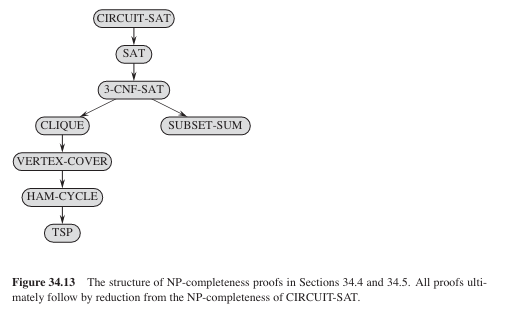
\includegraphics[scale=0.8]{graph.png}
\end{center}

Podemos decir que:

\begin{center}

    Lemma 1: $ V' \subseteq V $ es un certificado del problema.

    Lemma 2: 3-CNF-SAT $ \in $ NP-C

    Lemma 3: 3-CNF-SAT $ \leq_p $ CLIQUE
    
    Lemma 4: Esta prueba viene de la reducción de la prueba de NP-Completitud
    de Circuit-SAT

\end{center}
Dada la definición del problema y la figura 34.13[1], sabemos que este problema va a
ser lo que llamamos una reducción de mapeo, la cuál se define como la conversión de un
problema de decisión a otro, dada una reducción del problema. En este caso, sabemos que
de demostrar que Clique se puede reducir a 3-CNF-SAT, bajo las reglas establecidas en 
'Degrees of Computability' de Norman Shapiro [2] y anteriormente de otros autores dentro
del campo de las matemáticas discretas, donde se establece la capacidad de reducir problemas
dentro de otros de la forma:

\begin{center}
    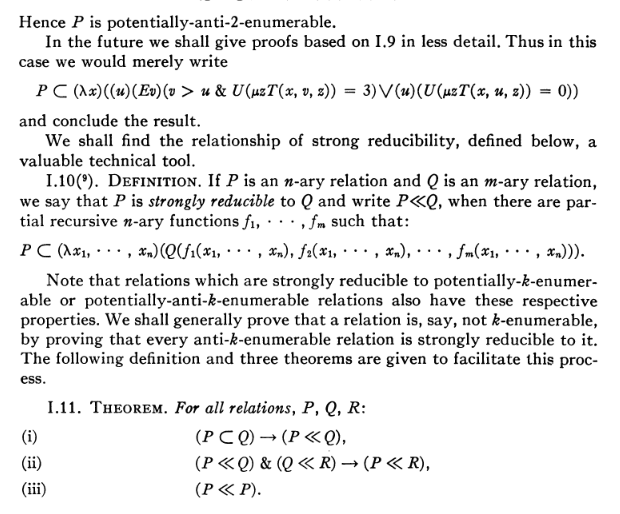
\includegraphics[scale=0.5]{Shabiro.png}    
\end{center}

que puede usarse en operaciones binarias, como sería el caso de Clique y de 3-CNF-SAT
por medio de pensarlas como conjuntos, entonces de poder reducir Clique a 3-CNF-SAT podremos
encontrar una prueba de que por medio del Lemma 2, entonces Clique $ \in $ NP-C. Dado esto,
Dentro de Cormen encontramos la capacidad de reducción del problema dada por medio de la 
construcción de un grafo 'G' que derivamos a partir de un certificado del problema 3-CNF-SAT.
definido de esta forma: 
\begin{center}
    \includegraphics*[scale=0.7]{gCNF3.png}
\end{center}

En este grafo, podemos ver 3 certificados del problema 3-SAT formando un grafo donde la condicion
de 3-CNF-SAT se satisface en el caso de que exista un clique de tamaño k, y al probar que la existencia
de dicho Clique hace satisfacer 3-CNF-SAT, podemos demostrar que $ P << Q $ para estos dos problemas.
En este caso, un clique de tamaño 3 (dado por medio del número de certificados a tener en cuenta) se 
ve reducible dada la capacidad de construir una solución de 3-CNF-SAT a partir de las siguientes cláusulas:

\begin{itemize}
    \item los elementos que nos permiten hacer el certificado estan en triplas diferentes (es decir, las conexiones estan establecidas de forma tal que el grafo tenga vertices que conectan de un certificado a otro pero no los elementos internamente dentro de un certificado). Esto se hace para poder garantizar que para esta solucion de k certificados, no se dependa de conexiones dentro de un mismo certificado y que todos los elementos se usen
    \item Un elemento no sea negación de otro, es decir, en casos como $ x_2 \land \lnot x_2  $ (el cual se evidencia dentro de este grafo) no se establece una conexión para evitar un caso en el que se llegue a un resultado ilógico, donde un valor booleano es True y False a la vez.
    \item todos los resultados estan conectados entre si, esto importa porque la definición de 'Clique' requiere un subgrafo con todos sus elementos interconectados entre sí y por lo tanto, para encontrar una reducción que satisface Clique, se debe mantener esta regla.
    \item 
\end{itemize}

Una vez se garantiza todo esto, podemos encontrar un grafo cuyos vertices son no dirigidos, y que, de haber una solución para 'Clique' dentro de
este, se podría a partir de dicha solucion derivar una respuesta a 3-CNF-SAT cuya forma se puede reducir por medio de la definición de 'P' y 'Q' del 
paper de Norman Shapiro. En el diagrama del grafo proveído, se puede encontrar esta solución al unir $ x_3(C_3) \land x_3(C_2) \land \lnot x_2(C_1) $
Este subgrafo esta fuertemente conectado como es requerido por Clique, y fuera de eso, al tomar los valores de sus nodos y colocarlos dentro de un certificado
para el problema a reducir, se encuentra una solución válida a la pregunta. Y cómo este grafo puede construirse en tiempo polinomial dadas las carácteristicas de
los problemas de tipo SAT (Tengamos en cuenta que cada evaluación de $ x_n $ se resuelve en tiempo constante O(1) y que por el Lemma 2 sabemos que todos los certificados
usados tendrían mas o menos la misma complejidad por pertenecer al mismo tipo de problema). Teniendo en cuenta todo esto, y que las definiciones se cumplen para las conexiones
establecidas dentro de este grafo. Entonces podemos establecer que $ x_3(C_3) \land x_3(C_2) \land \lnot x_2(C_1) $ es un certificado de la forma del Lemma 1 al tener
en cuenta sus vertices, y que podemos encontrar $ V' \subseteq V $ a partir de la construcción de este grafo a partir de certificados de 3-CNF-SAT.



\paragraph{Nota 1:} aunque no esta anotado en este taller, se puede comprobar la satisfacibilidad de 3-CNF-SAT
a partir de la reducción de circuit SAT y de la prueba de circuit SAT vista en clase. Simplemente es
cosa de que esto nos tomaría bastante tiempo para la hora de clase en la que se hace este taller.

\paragraph{Nota 2:} la complejidad total de clique es establecida dentro del libro de Cormen como $ O(k^2*(|V|/k)) $, que dado
el valor constante de la variable k, será tiempo polinomial dentro de este contexto, otra vez, no se demuestra por
cuestiones de tiempo dentro de este trabajo, mas allá de la mención del tiempo polinomial asumido para el problema
en el que se reduce, necesario para partir de la idea de que se puede reducir a un problema polinomial.


\subsection*{Bibliografía}
\begin{itemize}
    \item [1] Introduction to Algorithms, Cormen, 3rd edition.
    \item [2] Degrees of Computability, Norman Shapiro. recuperado de:
    
    https://web.archive.org/web/20180811065234/https://

    pdfs.semanticscholar.org/742b/cb582c02c9658888b8b4fb6191737a5c790c.pdf
\end{itemize}
\end{document}
CLIQUE